\chapter{Realisieren}
In diesem Kapitel geht es um die Implementation der Software. Diese wird nach den Diagrammen aus dem Kapitel
\ref{chap:plan}, Planen.

\section{Entwicklungsumgebung}
\subsection{Versionierung}
Für die Versionierung wird Git verwendet. Dabei wird GitHub als Remote-Repository verwendet. Das Repository mit
dem Source-Code kann unter \url{https://github.com/aneshodza/gnosis} gefunden werden.

\subsection{IDE}
Als IDE wird vim mit verschiedenen Plugins verwendet. Bestimmte Sachen wurden in der \bgmintinline{bash}{.vimrc} Datei
konfiguriert, damit die Arbeit möglichst effizient ist. \newline
Diese Konfigurationen sind unter \newline
\url{https://github.com/aneshodza/.dotfiles/blob/ad87ee9ecc5588a59d66e211797792099569ca95/.vimrc} zu finden.

\subsection{CI/CD}
Für die CI/CD Pipeline wird SemaphoreCI verwendet. Das ist passend, da auch die PA sehr eng mit SemaphoreCI verbunden
ist.

\begin{minipage}{\textwidth}
  \section{Aufsetzen des Projektes}
  Zu Beginn wird Arbeitspaket 7, Aufestzen des Projektes, implementiert. Dazu sind folgende Schritte zu befolgen:
  \begin{enumerate}
    \item Erstellen des Plugins
    \item Erstellen des Remote-Repository
    \item Mit dem README beginnen
    \item Aufsetzen der CI/CD Pipeline \newline
  \end{enumerate}
\end{minipage}

\begin{minipage}{\textwidth}
  \subsection{Erstellen des Plugins}
  Um das Plugin aufzusetzen begeben wir uns in das Verzeichnis der Lokalen Redmine Instanz. Diese wurde in den
  Vorarbeiten bereits erstellt und aufgesetzt. \newline
  Dort wird mit dem Befehl \bgmintinline{bash}{bundle exec rake generate redmine_plugin gnosis} das Plugin erstellt. Der
  Konsolen-Output sieht wie folgt aus:
  \begin{codebox}[]
    \begin{minted}{bash}
> bundle exec rails generate redmine_plugin gnosis
create  plugins/gnosis/app
# Lots of things being created...
create  plugins/gnosis/README.rdoc
# Lots of things being created...
create  plugins/gnosis/test/test_helper.rb
    \end{minted}
  \end{codebox}

  Wenn wir dann mit \bgmintinline{bash}{cd plugins/gnosis} in das Plugin wechseln, sehen wir, dass bestimmte Dateien
  bereits wurden. Diese werden bei Gebrauch erklärt und aufgezeigt.
\end{minipage}

\begin{minipage}{\textwidth}
  \subsection{Erstellen \& Konfigurieren des Repository}
  Das Projekt wird auf GitHub mit Git Versionsverwaltet, weshalb als Erstes ein GitHub Remote-Repository (auch einfach
  Repository genannt) erstellt werden muss. Das wird nach GitHub Dokumentation gemacht \cite{github_create_repo}.

  \subsubsection{Erstellen des Lokalen Repostiory}
  Danach muss das lokale Plugin mit dem Repository verbunden werden. Dazu müssen wir mit der Konsole in das Directory
  unseres Plugin wechseln, welches unter \menu{redmine/plugins/gnosis} zu finden ist. \newline
  Dort initialisieren wir das lokale Repository mit \bgmintinline{bash}{git init} und verbinden es mit dem Remote
  Repository indem wir \bgmintinline{bash}{git remote add origin [URL]} ausführen.

  \subsubsection{Initial Commit}
  Nun können wir den ersten Commit machen. Das können wir ganz einfach mit wenigen Befehlen machen:
  \begin{codebox}[]
    \begin{minted}{bash}
> git add -A
> git commit -m "Initial commit"
> git push -u origin main
    \end{minted}
  \end{codebox}

  \subsubsection{Git-flow initialisieren}
  Das Projekt wird nach der Git-flow Methode versioniert. Das bedeutet, dass der main Branch für die Releases
  verwendet wird und der develop Branch für die Entwicklung. \newline
  Dann hat man auch feature, bugfix und hotfix Branches, welche alle selbsterklärend sind. \newline
  Für jedes AP wird ein feature Branch erstellt, welcher dann in den develop Branch gemerged wird. \newline
  Als erstes müssen wir den develop branch mit \bgmintinline{bash}{git checkout -b develop} erstellen und diesen
  mit \bgmintinline{bash}{git push -u origin develop} auf remote pushen. \newline
\end{minipage}

\begin{minipage}{\textwidth}
  \subsection{Erstellen des README}
  Beim Erstellen des Plugins wurde automatisch ein \enquote{README.rdoc} erstellt. Dieses wird bei Ruby Projekten
  oft anstatt eines \enquote{README.md} verwendet. Da diese PA nach Vorgaben von Redmine arbeitet, wird auch das
  README im rdoc Format geschrieben. \newline
  Da noch nicht viel im Projekt steht, wird nur beschrieben was genau das Plugin kann und wie es funktioniert. \newline
\end{minipage}

\subsection{Aufsetzen der CI/CD Pipeline}
Die CI/CD wird auf SemaphoreCI eingerichtet, weshalb wir uns dort anmelden und ein neues Projekt erstellen. Man kann dieses
direkt mit GitHub verbinden und Semaphore die meiste Arbeit machen lassen.

\subsubsection{Erstellen der \enquote{bin files}}
Da die Tests sowie Linter immer wieder ausgeführt werden, ist es sinnvoll diesen Prozess zu automatisieren. Dazu werden 
\enquote{bin files} erstellt. Diese sind kleine Bash-Scripts, welche repeditive Aufgaben automatisieren. In unserem Fall sind
das die Ausführungen von den Tests und Lintern sowie das aufsetzen des Projektes. \newline

\begin{minipage}{\textwidth}
  Für die Tests wird ein \bgmintinline{bash}{bin/test} mit folgendem Inhalt erstellt:
  \begin{codebox}[]
    \begin{minted}{bash}
#!/bin/bash

white='\033[1;37m'
red='\033[0;31m'
green='\033[0;32m'

rake redmine:plugins:test

if [[ $? -eq 0 ]]; then
  echo -e "${green}----------------------------------------"
  echo -e "Tests passed"
  echo -e "----------------------------------------${white}"
else
  echo -e "${red}----------------------------------------"
  echo -e "Tests failed"
  echo -e "----------------------------------------${white}"
  exit 1
fi
    \end{minted}
  \end{codebox}
\end{minipage}

\begin{minipage}{\textwidth}
  Dann braucht es ein \bgmintinline{bash}{bin/fastcheck} für linter und so weiter mit folgendem Inhalt:
  \begin{codebox}[]
    \begin{minted}{bash}
#!/bin/bash

white='\033[1;37m'
red='\033[0;31m'
green='\033[0;32m'

function return_code {
  if [ $? -ne 0 ]; then
    echo -e "${red} Error: $1 found errors! ${white}"
    failing_checks+=("$1")
    passing=false
  fi
}

passing=true
failing_checks=()

echo "Executing fastchecks..."

if [[ $* == *--fix* ]]; then
  echo "Fixing..."
  bundle exec rubocop -a --config .rubocop.yml
  return_code "Rubocop"
else 
  echo "Note: You can use --fix to fix the errors automatically"
  bundle exec rubocop --config .rubocop.yml
  return_code "Rubocop"
fi

bundle exec brakeman -q -z --no-summary --no-pager
return_code "Brakeman"

if [ "$passing" = true ]; then
  echo -e "${green}----------------------------------------"
  echo -e "All checks passed"
  echo -e "----------------------------------------${white}"
  exit 0
  else
  echo -e "${red}----------------------------------------"
  echo -e "Some checks failed"
  echo -e "Failed checks: ${failing_checks[@]}"
  echo -e "----------------------------------------${white}"
  exit 1
fi
    \end{minted}
  \end{codebox}
  
\end{minipage}

\begin{minipage}{\textwidth}
  Dann braucht es ein \bgmintinline{bash}{bin/setup} für das aufsetzen des Projektes mit folgendem Inhalt:
  \begin{codebox}[]
    \begin{minted}{bash}
yarn install
bundle exec rake redmine:plugins:migrate
    \end{minted}
  \end{codebox}
\end{minipage}

\subsubsection{Erstellen der \enquote{semaphore.yml} Datei}
Was wir noch machen müssen, ist die \bgmintinline{bash}{semaphore.yml} Datei zu erstellen. Diese muss ungefähr folgenden Ablauf
ausführen:
\begin{enumerate}
  \item Redmine klonen und Aufsetzen
  \item Postgres starten
  \item Datenbank erstellen und migrieren
  \item In das Plugins directory wechseln
  \item Plugin klonen
  \item Tests ausführen
\end{enumerate}

\begin{minipage}{\textwidth}
  Auf einem Activity Diagramm würde das so aussehen: \newline
  \begin{center}
    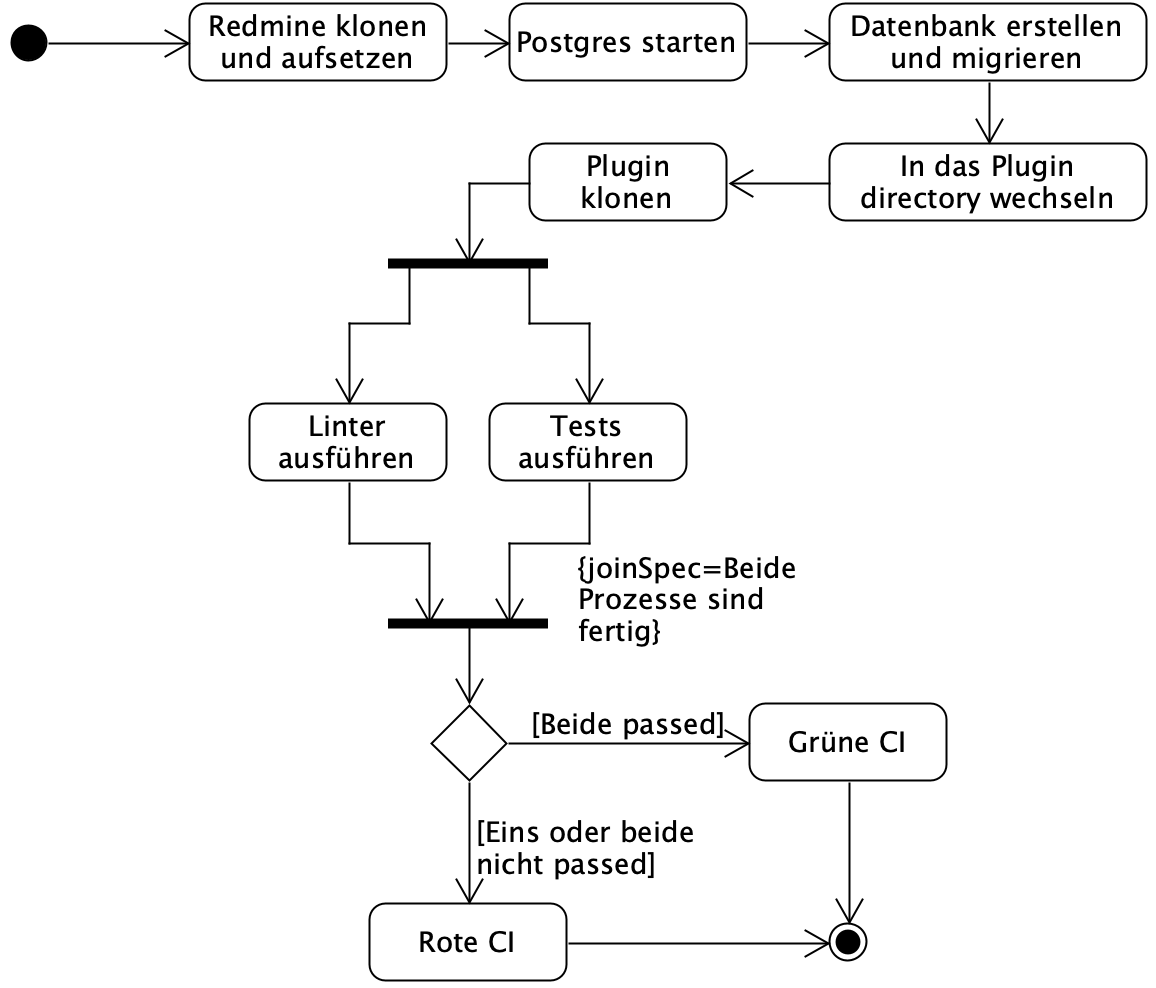
\includegraphics[width=0.8\textwidth]{images/activity/ci-cd.png}
    \label{fig:activity_ci_cd}
    \newline
  \end{center}
\end{minipage}

\begin{minipage}{\textwidth}
  Die oben beschriebene semaphore.yml Datei sieht dann so aus:
  \begin{codebox}[]
    \begin{minted}{yaml}
version: v1.0
name: Initial Pipeline
agent:
  machine:
    type: e1-standard-2
    os_image: ubuntu2004
blocks:
  - name: Checks
    task:
      jobs:
        - name: Tests
          commands:
            - bin/test
        - name: Linter
          commands:
            - bin/fastcheck
      prologue:
        commands:
          - 'git clone git@github.com:redmine/redmine.git'
          - cd redmine
          - cp config/configuration.yml.example config/configuration.yml
          - 'git clone git@github.com:aneshodza/redmine-postgres-database-yml.git'
          - cp redmine-postgres-database-yml/database.yml config/database.yml
          - rm -rf redmine-postgres-database-yml
          - bin/bundle install
          - yarn
          - sem-service start postgres --username="root" --password=""
          - 'bin/rails db:create'
          - 'bin/rails db:migrate'
          - cd plugins
          - checkout
          - cd ../../
          - bin/bundle install
          - cd plugins/gnosis
          - bin/setup
    \end{minted}
  \end{codebox}
  \textbf{Wichtig:} Auf Zeile 22 wird von einem Repository geklont. Das hat den Grund, dass das
  \bgmintinline{bash}{database.example.yml} nicht mit der MySQL Version von SemaphoreCI kompatibel ist. Das führt dazu,
  dass die Migrationen nicht durchlaufen können, wie in diesem StackOverflow issue beschrieben: \newline
  \url{https://stackoverflow.com/questions/63158705/rails-migration-mysql2error-specified-key-was-too-long-max-key-length-is-7}
  \newline
  Deswegen wird eine eigene Datenbank-Konfiguration verwendet.
\end{minipage}

\begin{minipage}{\textwidth}
  Nachdem das alles erledigt wurde, wird schnell ersichtlich, ob alles richtig ist oder nicht. In diesem Fall soll die CI
  grün sein: \newline
  \begin{center}
    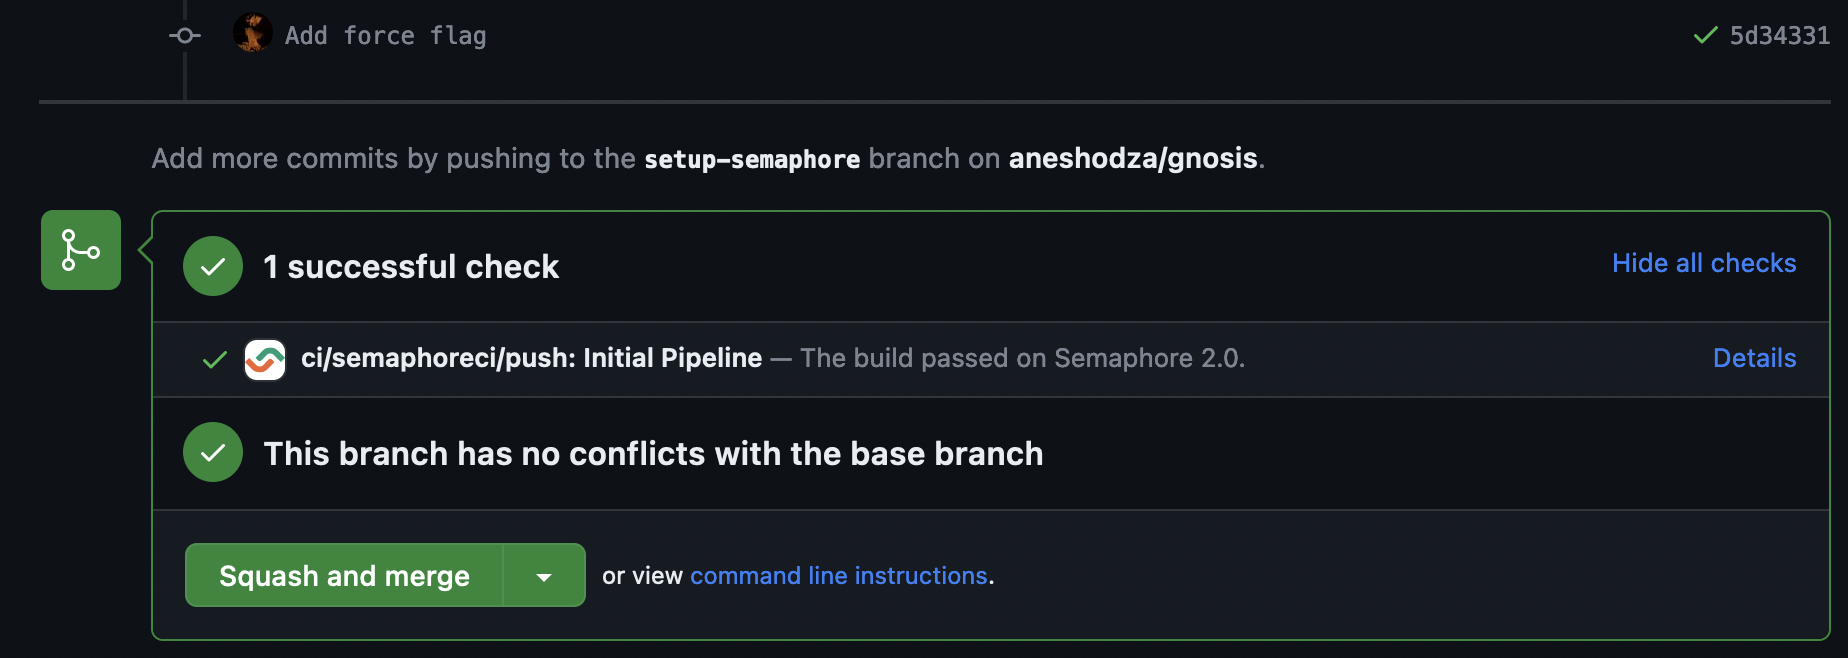
\includegraphics[width=0.8\textwidth]{images/misc/ci-passed.png}
    \label{fig:semaphore_ci_passed}
    \newline
  \end{center}
\end{minipage}

\begin{minipage}{\textwidth}
  \section{Umsetzung der Datenstruktur}
  Da unter Kapitel \ref{sec:decide_erd} die Entscheidung getroffen wurde die \enquote{has many trough} Beziehung zu
  verwenden, wird diese auch implementiert. Das bedeutet, dass wir zwei Objekte erstellen müssen: 
  \bgmintinline{ruby}{PullRequest} und \bgmintinline{ruby}{Deployment}. Diese muss man mit dem Redmine CLI generieren,
  damit die neuen Objekte richtig mit den anderen Objekten von Redmine interagieren können. Für das Generieren unserer
  Objekte muss man folgende Befehle ausführen:
  \begin{codebox}[]
    \begin{minted}{bash}
rails generate redmine_plugin_model gnosis PullRequest 
rails generate redmine_plugin_model gnosis Deployment
rake redmine:plugins:migrate
    \end{minted}
  \end{codebox}
  \textbf{Wichtig:} Die Migrationen wurden noch mit den Attributen aus dem ERD befüllt. \newline
  Um dann die Associations nach Rails Standard zu machen, müssen wir unsere neuen Objekte wie folgt anpassen:
  \begin{codebox}[]
    \begin{minted}{ruby}
class PullRequest < ActiveRecord::Base
  belongs_to :issue
  has_many :deployments, dependent: :destroy
end

class Deployment < ActiveRecord::Base
  belongs_to :pull_request
  has_one :issue, through: :pull_request
end
    \end{minted}
  \end{codebox}
\end{minipage}

